\documentclass[conference]{IEEEtran}
\IEEEoverridecommandlockouts
% The preceding line is only needed to identify funding in the first footnote. If that is unneeded, please comment it out.
\usepackage{cite}
\usepackage{amsmath,amssymb,amsfonts}
\usepackage{algorithmic}
\usepackage{graphicx}
\graphicspath{{Imgs/}}
\usepackage{textcomp}
\usepackage{xcolor}
\usepackage{hyperref}
\usepackage{multicol}
\usepackage{listings}
\usepackage{color}
\lstloadlanguages{C,C++,csh,Java}

\definecolor{red}{rgb}{0.6,0,0} 
\definecolor{blue}{rgb}{0,0,0.6}
\definecolor{green}{rgb}{0,0.8,0}
\definecolor{cyan}{rgb}{0.0,0.6,0.6}

\lstset{
language=csh,
basicstyle=\footnotesize\ttfamily,
numbers=left,
numberstyle=\tiny,
numbersep=5pt,
tabsize=2,
extendedchars=true,
breaklines=true,
frame=b,
stringstyle=\color{blue}\ttfamily,
showspaces=false,
showtabs=false,
xleftmargin=17pt,
framexleftmargin=17pt,
framexrightmargin=5pt,
framexbottommargin=4pt,
commentstyle=\color{green},
morecomment=[l]{//}, %use comment-line-style!
morecomment=[s]{/*}{*/}, %for multiline comments
showstringspaces=false,
morekeywords={ abstract, event, new, struct,
as, explicit, null, switch,
base, extern, object, this,
bool, false, operator, throw,
break, finally, out, true,
byte, fixed, override, try,
case, float, params, typeof,
catch, for, private, uint,
char, foreach, protected, ulong,
checked, goto, public, unchecked,
class, if, readonly, unsafe,
const, implicit, ref, ushort,
continue, in, return, using,
decimal, int, sbyte, virtual,
default, interface, sealed, volatile,
delegate, internal, short, void,
do, is, sizeof, while,
double, lock, stackalloc,
else, long, static,
enum, namespace, string},
keywordstyle=\color{cyan},
identifierstyle=\color{red},
backgroundcolor=\color{cloudwhite},
}
\usepackage{caption}
\DeclareCaptionFont{white}{\color{white}}
\DeclareCaptionFormat{listing}{\colorbox{blue}{\parbox{\textwidth}{\hspace{15pt}#1#2#3}}}
\captionsetup[lstlisting]{format=listing,labelfont=white,textfont=white, singlelinecheck=false, margin=0pt, font={bf,footnotesize}}
\definecolor{cloudwhite}{rgb}{0.9412, 0.9608, 0.8471} 




\renewcommand{\abstractname}{Abstracto}
\def\BibTeX{{\rm B\kern-.05em{\sc i\kern-.025em b}\kern-.08em
    T\kern-.1667em\lower.7ex\hbox{E}\kern-.125emX}}
\begin{document}
\renewcommand\IEEEkeywordsname{Palabras clave}

{\footnotesize 
\title{Motor de encadenamientos.}
}

\author{
\IEEEauthorblockN{García García Jonathan Eduardo}
\IEEEauthorblockA{\href{mailto:jgarciag1404@alumno.ipn.mx}{jgarciag1404@alumno.ipn.mx}}
\and
\IEEEauthorblockN{González Santiesteban Santiago}
\IEEEauthorblockA{\href{mailto:sgonzalezs1400@alumno.ipn.mx}{sgonzalezs1400@alumno.ipn.mx}}
\and
\IEEEauthorblockN{Jimenez Angeles Daniel Antonio}
\IEEEauthorblockA{\href{mailto:djimeneza1400@alumno.ipn.mx}{djimeneza1400@alumno.ipn.mx}}
}

\maketitle

\begin{abstract}
Este documento es el reporte técnico, explicativo de la estructura interna de este motor de encadenamientos.
\end{abstract}

\begin{IEEEkeywords}
Encadenamiento, inferencia, sistema experto, toma de decisiones
\end{IEEEkeywords}

\section{Introducción}
Un motor de inferencia es el encargado de manejar el proceso de selección, decisión, 
interpretación y aplicación del comportamiento que refleja el razonamiento.
 Procesa e interpreta reglas que se encargan de resolver un problema de decisión. 
 En la lógica clásica, es posible deducirse mediante el empleo de reglas, si su premisa es 
 cierta, también lo será su conclusión. 
\section{Marco teórico}

\subsection{Sistema experto}
Se puede decir que los Sistemas Expertos son el primer resultado operacional de la Inteligencia
 artificial, pues logran resolver problemas a través del 
 conocimiento y raciocinio de igual forma que lo hace el experto humano. 
 Un Sistema Experto (SE), es básicamente un programa de 
 computadora basado en conocimientos y raciocinio que lleva a cabo tareas que 
 generalmente sólo realiza un experto humano9; es decir, es un programa que 
 imita el comportamiento humano en el sentido de que utiliza la información 
 que le es proporcionada para poder dar una opinión sobre un tema en 
 especial. Otros autores lo definen como sigue:\\ un Sistema Experto es un programa 
 de computadora interactivo que contiene la experiencia, conocimiento y 
 habilidad propios de una persona o grupos de personas especialistas 
 en un área particular del conocimiento humano, de manera que permitan 
 resolver problemas específicos de ése área de manera inteligente y 
 satisfactoria10. La tarea principal de un SE es tratar de aconsejar al usuario. 
 Los usuarios que introducen la información al SE son en realidad los 
 expertos humanos, y tratan a su vez de estructurar los conocimientos 
 que poseen para ponerlos entonces a disposición del sistema. Los SE 
 son útiles para resolver problemas que se basan en conocimiento. 
\begin{figure}[h!]
    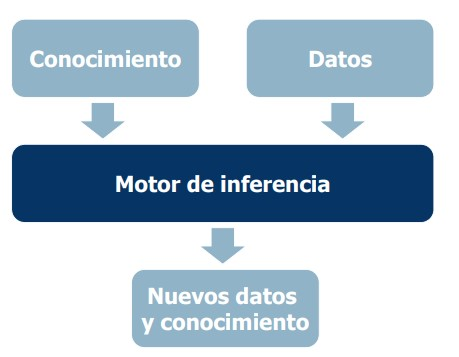
\includegraphics[height=4cm]{sistemae.jpg}
\end{figure}

\subsection{Modus Ponens}
Es quizá la regla de inferencia más comúnmente utilizada. Se utiliza para obtener conclusiones simples, en ella se analiza la premisa de la regla, y si es cierta, la conclusión entra a formar parte del conocimiento. Como ilustración supóngase que se tiene la regla, “Si A es cierto, entonces B es cierto”, y que se sabe además que “A es cierto”. La regla Modus Ponens, concluye que “B es cierto”.
\\
\begin{figure}[h!]
    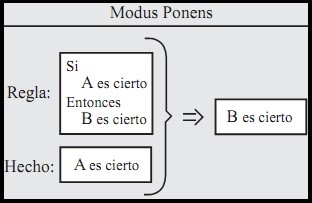
\includegraphics[height=4cm]{modus.jpg}
\end{figure}

\subsection{Arquitectura de un sistema experto}
\begin{figure}[h!]
    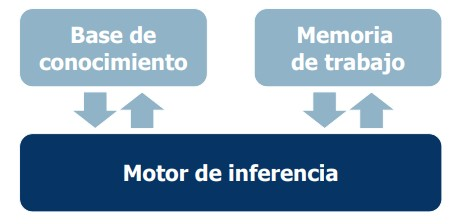
\includegraphics[height=4cm]{arquitectura.jpg}
\end{figure}


\section{Desarrollo}
El motor de inferencia están escritos en C\# "C Sharp" debido a que este lenguaje de programación implementa los pilares de \textbf{POO}.
\begin{itemize}
    \item \textbf{Abstracción}\\ 
    Permite diseñar cada uno de los modulos de un microprocesador a nivel de objetos.
    \item \textbf{Polimorfismo}\\
    Permite sobrecargar métodos teniendo un único patrón en conmún.
    \item \textbf{Encapsulamiento}\\
     Protege los datos almacenados en la memoria limitando la lectura ó escritura de los mismos a menos que seán autorizados explicitamente.
    \item \textbf{Herencia}\\
    Permite compartir fragmentos de código entre clases heredando métodos y atributos evitando la redundacia en el código.
\end{itemize}

\subsection{Generalidades}
El programa permite definir y ejecutar las estrucutras de Encadenamiento hacia adelante y hacia atras
Entre los módulos implementados para cumplir con el objetivo se encuentran:

\begin{itemize}
    \item Definición y edición de encadenamiento hacia adelante
    \item Definición y edición de encadenamiento hacia atrás.
    \item Base de datos de sqlite (donde se almacena la base de conocimiento)
    \item Interfaz de ejecución de encadenamiento hacia adelante
    \item Interfaz de ejecución de encadenamiento hacia atras
\end{itemize}

\section{Proceso de Ejecución}
Seleccionar el encadenamiento que se desea ejecutar:
\\
\begin{figure}[h!]
    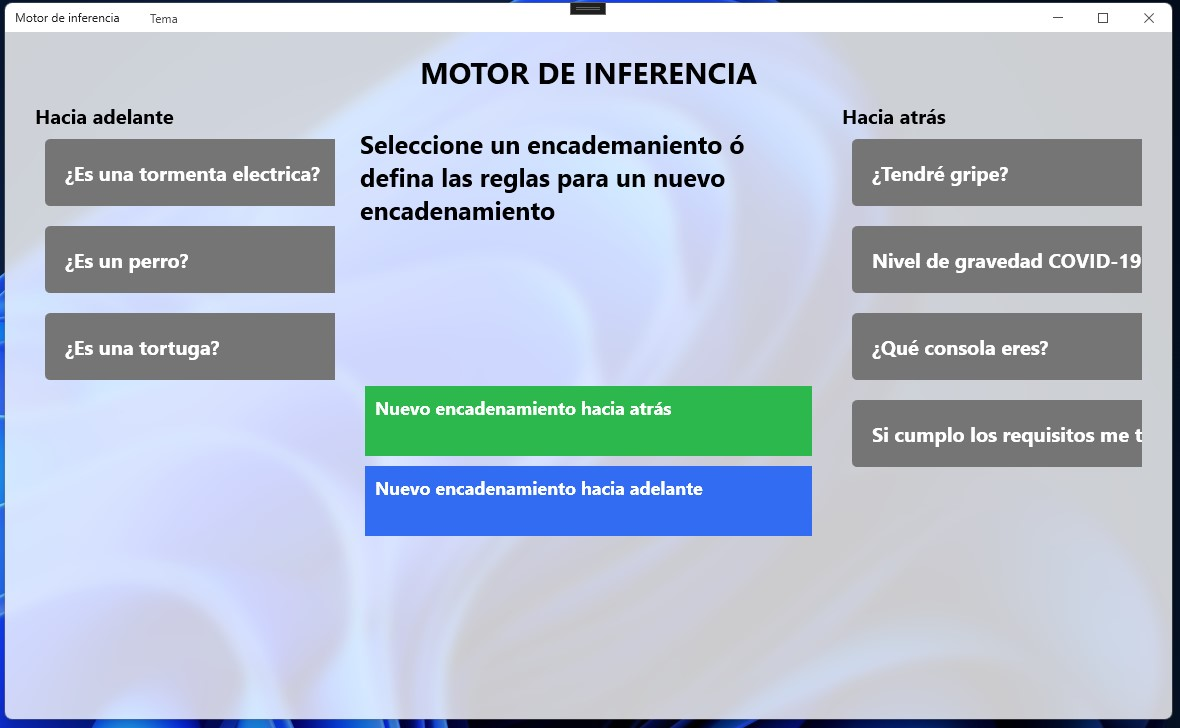
\includegraphics[width=8cm]{principal.jpg}
\end{figure}
\\
Encadenamiento hacia adelante:
\begin{figure}[h!]
    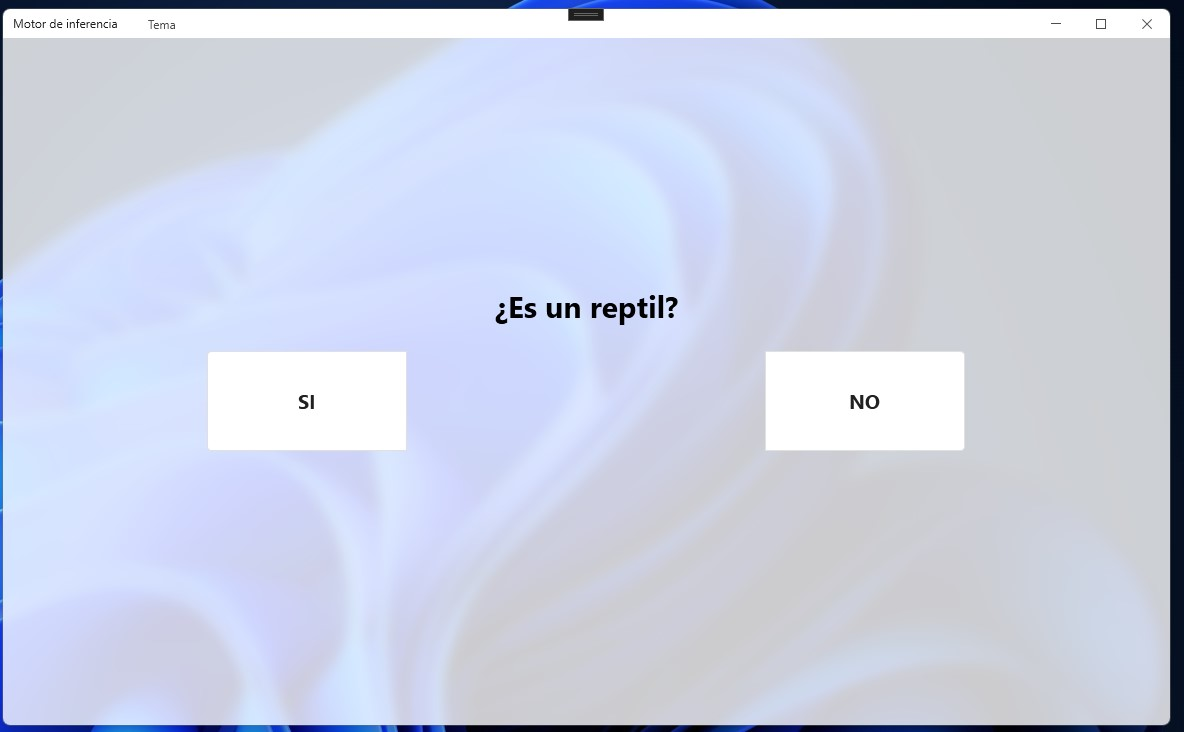
\includegraphics[width=7cm]{ejecucionadelante.jpg}
\end{figure}
\newpage
Encadenamiento hacia atrás:
\begin{figure}[h!]
    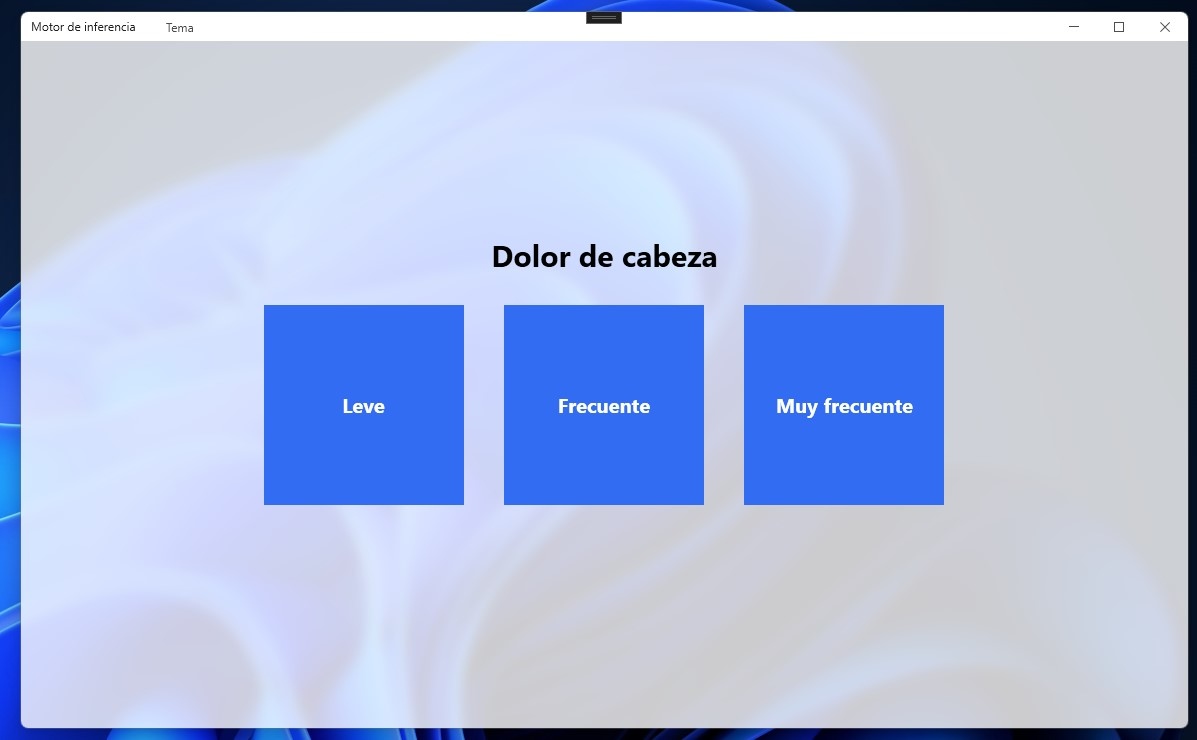
\includegraphics[width=8cm]{ejecucionatras.jpg}
\end{figure}
Definición y edición de encadenamiento hacia atrás:
\begin{figure}[h!]
    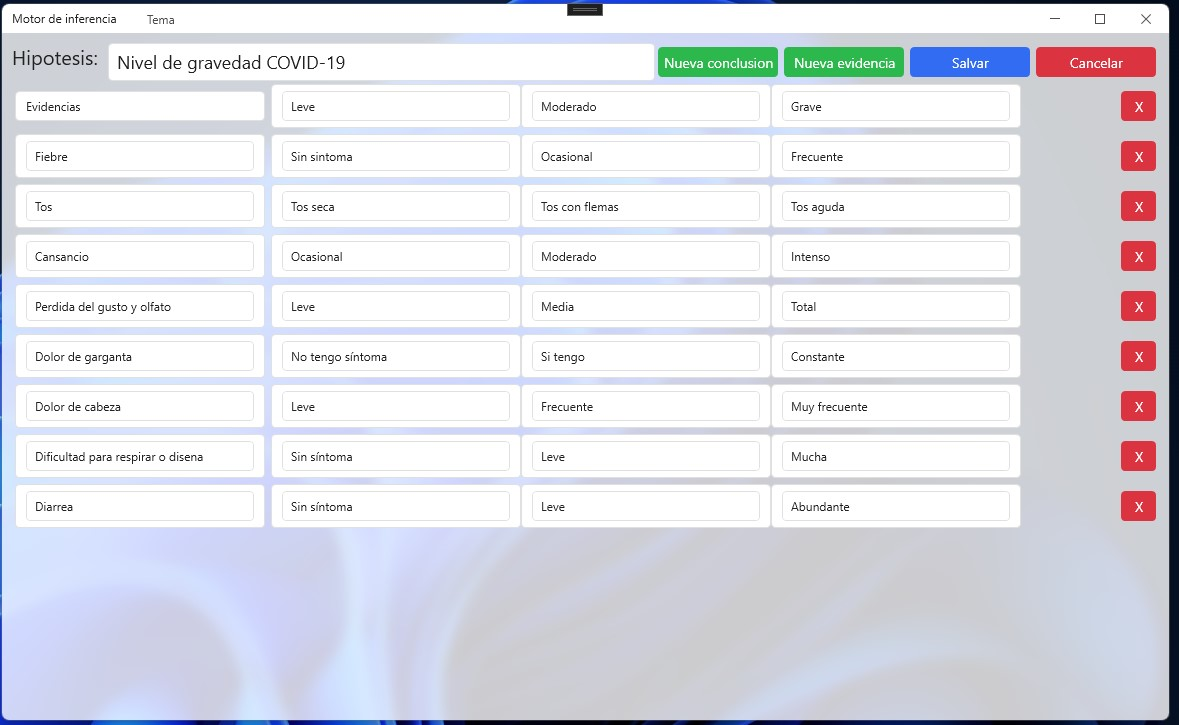
\includegraphics[width=8cm]{hacia_atrasjpg.jpg}
\end{figure}

Definición y edición de encadenamiento hacia adelante:
\begin{figure}[h!]
    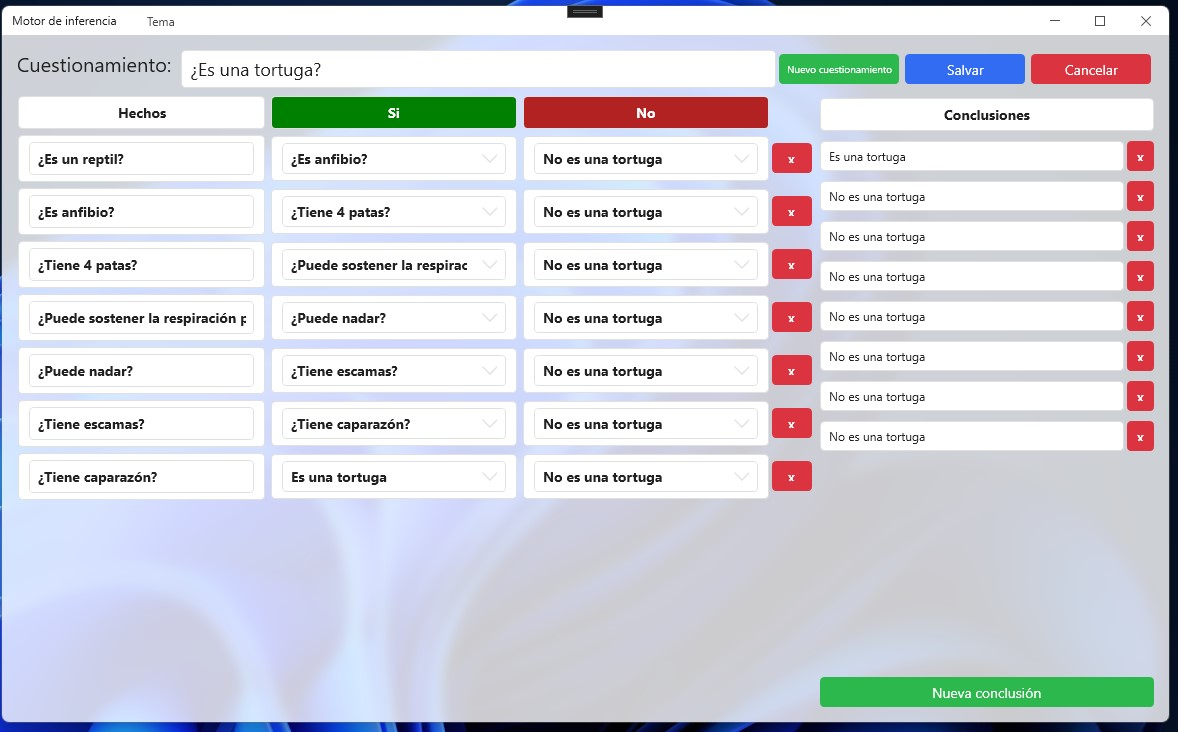
\includegraphics[width=8cm]{hacia_adelante.jpg}
\end{figure}
\newpage

\begin{figure*}[t]
    \section{Código de las clases principales}
\subsection{IQuestion}    
\begin{lstlisting}[language={[Sharp]C}, title={IQuestion}]
    public interface IQuestion
    {
        public bool Answer { get; set; }
        public string Question { get; set; }
        public void Ask(MainView mainView);
    }
\end{lstlisting}
\end{figure*}
\newpage

\begin{figure*}[t]
\subsection{IEncadenamiento}   
\begin{lstlisting}[language={[Sharp]C}, title={IEncadenamiento}]
    public interface IEncadenamiento
    {
        [JsonIgnore]
        public string Title { get; }
        [JsonIgnore]
        public string Type { get; }
    }
\end{lstlisting}
\end{figure*}

\newpage
\begin{figure*}[t]
    \subsection{Engine}
    \begin{lstlisting}[language={[Sharp]C}, title={Engine}]
        public static class Engine
        {
            public static void Run(MainView mainView, IEncadenamiento encadenamiento)
            {
                switch (encadenamiento)
                {
                    case HaciaAtras atras:
                        Run(mainView, atras.Hipotesis);
                        return;
                    case HaciaAdelante adelante:
                        Run(mainView, adelante.Hecho);
                        return;
                }
            }
            public static void Run(MainView mainView, Atras.Hipotesis hipotesis)
            {
                mainView.Content = new StartupView(new StartupViewModel(mainView, hipotesis));
            }
            public static void Run(MainView mainView, Adelante.Hecho hecho)
            {
                mainView.Content = new StartupView(new StartupViewModel(mainView, hecho));
            }
        }
\end{lstlisting}
\end{figure*}
\newpage 

\begin{figure*}[t]
    \subsection{Conclusion}
\begin{lstlisting}[language={[Sharp]C}, title={Conclusion}]
    public class Conclusion : IGuid, IComparable<Conclusion>, IEquatable<Conclusion>, IBranch
    {
        public string Descripcion { get; set; }
        [PrimaryKey]
        public Guid Guid { get; set; }
        public bool Side { get; set; }
        public Guid ParentId { get; set; }
        public Conclusion()
        {

        }
        public Conclusion(string descripcion)
        {
            Descripcion = descripcion;
        }
        public static Conclusion New(string descripcion) => new Conclusion(descripcion);

        public void Run(MainView window)
        {
            var view = new ConclusionView();
            var model = new ConclusionViewModel(window, this);
            view.DataContext = model;
            window.Content = view;
        }

        public void Delete()
        {
            App.SqLite.Delete(this);
        }
        public void Save()
        {
            App.SqLite.InsertOrReplace(this);
        }

        public void Save(Guid Guid, bool answer)
        {
            if (ParentId != Guid.Empty)
            {
                this.Guid = Guid.NewGuid();
            }
            ParentId = Guid;
            Side = answer;
            Save();
        }

        public void Load()
        {
            //nada que cargar :)
        }

        public bool Equals(Conclusion other)
        {
            return other?.Guid == this.Guid;
        }

        public override int GetHashCode()
        {
            var a = this.Guid.GetHashCode();
            return a;
        }

        public override string ToString() => Descripcion;

        public int CompareTo([AllowNull] Conclusion other) => this.Guid.CompareTo(other?.Guid ?? Guid.Empty);
    }
\end{lstlisting}
\end{figure*}
\newpage

\begin{figure*}[t]
    \subsection{Hipotesis}
\begin{lstlisting}[language={[Sharp]C}, title={Hipotesis}]
    public class Hipotesis : IQuestion, IBranch, IGuid
    {
        [PrimaryKey]
        public Guid Guid { get; set; }
        [Ignore]
        public bool Answer { get; set; }
        [Ignore]
        public string Descripcion => Question;
        public string Question { get; set; }
        [Ignore]
        public IBranch Verdadero { get; set; }
        [Ignore]
        public IBranch Falso { get; set; }
        public bool Side { get; set; }
        public Guid ParentId { get; set; }

        public new static Hipotesis New(string descripcion) => new Hipotesis(descripcion);
        public Hipotesis(string question)
        {
            Question = question;
        }

        public Hipotesis()
        {
            
        }

        public Hipotesis Set(IBranch verdadero, IBranch falso)
        {
            Verdadero = verdadero;
            Falso = falso;
            return this;
        }

        public void Run(MainView main) => Ask(main);
        public void Ask(MainView main)
        {
            var view = new QuestionView();
            var model = new QuestionViewModel(main, this);
            view.DataContext = model;
            main.Content = view;
        }

        public void Delete()
        {
            App.SqLite.Delete(this);
            this.Verdadero.Delete();
            this.Falso.Delete();
        }
        public void Save() => Save(Guid.Empty, false);

        public void Save(Guid pGuid, bool answer)
        {
            ParentId = pGuid;
            Side = answer;
            App.SqLite.InsertOrReplace(this);
            this.Verdadero.Save(Guid, true);
            this.Falso.Save(Guid, false);
        }

        public void Load()
        {

            this.Verdadero=(IBranch)
                App.SqLite.Table<Hipotesis>().FirstOrDefault(x => x.ParentId == this.Guid && x.Side)
                ?? App.SqLite.Table<Conclusion>().First(x => x.ParentId == this.Guid && x.Side);

            this.Falso = (IBranch)
                             App.SqLite.Table<Hipotesis>().FirstOrDefault(x => x.ParentId == this.Guid && !x.Side)
                             ?? App.SqLite.Table<Conclusion>().First(x => x.ParentId == this.Guid && !x.Side);
            this.Verdadero.Load();
            this.Falso.Load();

        }
    }
\end{lstlisting}
\end{figure*}

\end{document}
